\chapter{Programming}
\section{Hardware Description Languages}
\subsection{Abstraction Levels}
The purpose of using different abstraction levels is to hide details which are not essential for the current view of the problem. Information that is not important is hidden in higher levels of abstraction. The different abstraction levels of HDLs are shown in figure \ref{fig:hdlabstractionlevels}.
\begin{figure}[htbp]
\begin{center}
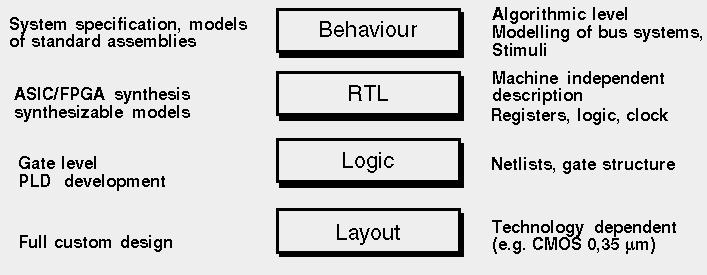
\includegraphics[width=10cm,keepaspectratio=true]{bilder/png/hdlabstractionlevels}
\caption{Abstraction levels of a HDL \cite{Ver16}}
\label{fig:hdlabstractionlevels}
\end{center}
\end{figure}
\subsubsection{Behavioural Level}
\subsubsection{Register-Transfer Level}
\subsubsection{Logical Level}
\subsubsection{Layout Level}
\label{kap:HDL}
\subsection{VHDL}
\subsection{Verilog}